\begin{figure}[htbp]
    \centering
    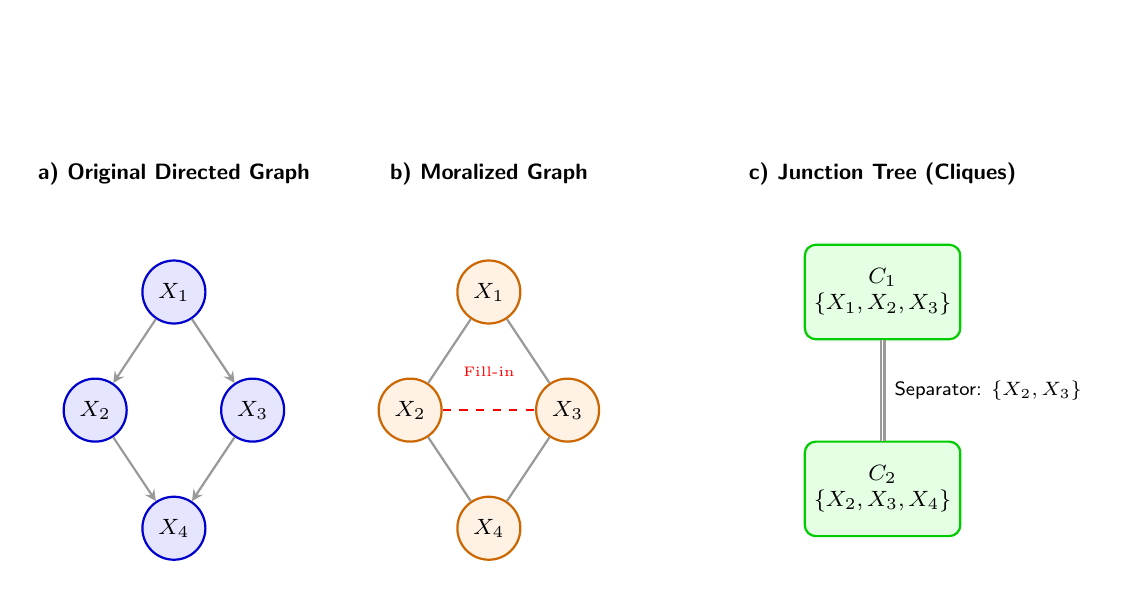
\begin{tikzpicture}[
        node distance = 1.2cm and 1.5cm,
        every node/.style = {
            draw, 
            circle, 
            align=center, 
            minimum size=0.8cm, 
            font=\sffamily\footnotesize
        },
        original/.style = {fill=blue!10, draw=blue!80!black, thick},
        moral/.style = {fill=orange!10, draw=orange!80!black, thick},
        clique/.style = {fill=green!10, draw=green!80!black, thick, rectangle, rounded corners, minimum height=1.2cm, minimum width=1.5cm},
        edge/.style = {-, thick, draw=gray!80},
        moral_edge/.style = {-, thick, draw=red, dashed},
        arrow/.style = {->, >=stealth, thick, draw=gray!80}
    ]

    % Panel A: Grafo Dirigido Original
    \node[draw=none] (titleA) at (0, 1.5) {\textbf{a) Original Directed Graph}};
    \node[original] (A1) at (0, 0) {$X_1$};
    \node[original] (A2) at (-1, -1.5) {$X_2$};
    \node[original] (A3) at (1, -1.5) {$X_3$};
    \node[original] (A4) at (0, -3) {$X_4$};
    
    \draw[arrow] (A1) -- (A2);
    \draw[arrow] (A1) -- (A3);
    \draw[arrow] (A2) -- (A4);
    \draw[arrow] (A3) -- (A4);

    % Panel B: Grafo Moralizado
    \node[draw=none] (titleB) at (4, 1.5) {\textbf{b) Moralized Graph}};
    \node[moral] (B1) at (4, 0) {$X_1$};
    \node[moral] (B2) at (3, -1.5) {$X_2$};
    \node[moral] (B3) at (5, -1.5) {$X_3$};
    \node[moral] (B4) at (4, -3) {$X_4$};
    
    \draw[edge] (B1) -- (B2);
    \draw[edge] (B1) -- (B3);
    \draw[edge] (B2) -- (B4);
    \draw[edge] (B3) -- (B4);
    % Enlace moral: casando a los padres de X4
    \draw[moral_edge] (B2) -- (B3) node[midway, above, draw=none, font=\tiny, text=red] {Fill-in};

    % Panel C: Árbol de Cliques (Junction Tree)
    \node[draw=none] (titleC) at (9, 1.5) {\textbf{c) Junction Tree (Cliques)}};
    
    \node[clique] (C1) at (9, 0) {$C_1$\\$\{X_1, X_2, X_3\}$};
    \node[clique] (C2) at (9, -2.5) {$C_2$\\$\{X_2, X_3, X_4\}$};
    
    \draw[edge, double] (C1) -- (C2) node[midway, right, draw=none, font=\sffamily\scriptsize] {Separator: $\{X_2, X_3\}$};

    \end{tikzpicture}
    \caption{\textbf{Classical Compilation Process (Junction Tree) and Treewidth Explosion.} \textbf{a)} A causal network featuring interdependent variables (e.g., photochemical reactions). \textbf{b)} Moralization requires "marrying" the parents ($X_2, X_3$) of the child node ($X_4$), introducing undirected fill-in edges. \textbf{c)} The resulting triangulation groups variables into large subsets known as cliques. The memory footprint scales exponentially with the size of the largest clique ($w = 2$ in this simplified schematic), precipitating RAM saturation in dense networks.}
    \label{fig:junction_tree_process}
\end{figure}
